\documentclass[12pt,oneside]{article}
\usepackage[utf8]{inputenc}
\usepackage{float}
\usepackage[bottom]{footmisc}
\usepackage{bookmark}
\usepackage{microtype}
\usepackage{amsmath}
\usepackage{multicol}
\usepackage{mdframed}
\usepackage{setspace}
\usepackage{pgfplots}
\usepackage{graphicx}
\usepackage[absolute]{textpos}\TPGrid{16}{16}
\usepackage{tikz}
  \usetikzlibrary{shapes}
  \usetikzlibrary{arrows}
  \usetikzlibrary{shadows}
  \usetikzlibrary{trees}
  \usetikzlibrary{fit}
  \usetikzlibrary{calc}
  \usetikzlibrary{positioning}
  \usetikzlibrary{decorations.pathmorphing}
\usepackage{everypage}
  \AddEverypageHook{
    \begin{textblock}{0.5}[0,0](0,0)
      \tikz \node[fill=myred,minimum width=0.5\TPHorizModule,minimum height=16\TPVertModule] {};
    \end{textblock}
    \begin{textblock}{0.125}[0,0](0.5,0)
      \tikz \node[fill=myblack,inner sep=0, minimum width=0.125\TPHorizModule,minimum height=16\TPVertModule] {};
    \end{textblock}
  }
\usepackage{xcolor}
  \definecolor{firebrick}{HTML}{B22222}
  \definecolor{myred}{HTML}{CF0A2C}
  \definecolor{myblack}{HTML}{232527}
\newcommand\dd[1]{\colorbox{gray!30}{\texttt{#1}}}
\usepackage{hyperref}
  \hypersetup{colorlinks=true,allcolors=blue!40!black}
\setlength{\topskip}{6pt}
\setlength{\parindent}{0pt} % indent first line
\setlength{\parskip}{6pt} % before par
% \let\oldsection\section\renewcommand\section{\newpage\oldsection}
\date{\small\today}
\title{%
  Binary Repository Manager\\
  \colorbox{firebrick}{\small\sffamily\color{white}{White Paper}}}
\usepackage[style=authoryear,sorting=nyt,backend=biber,
  hyperref=true,abbreviate=true,
  maxcitenames=1,maxbibnames=1]{biblatex}
  \renewbibmacro{in:}{}
  \addbibresource{books.bib}
\tikzset{node distance=1.6cm, auto, every text node part/.style={align=center, font={\sffamily\small}}}
\tikzstyle{block} = [draw=myblack, fill=white, inner sep=0.3cm, outer sep=0.1cm, thick]
\tikzstyle{ln} = [draw, ->, very thick, arrows={-triangle 90}, every text node part/.append style={font={\sffamily\scriptsize}}]
\begin{document}
\raggedbottom

\maketitle
\begin{abstract}
A software project of almost any size needs to keep its binary artifacts
in a repository, to enable access to them by programmers, tools, and other teams.
The quality of the software that manages the repository matters. There are
a few categories of such a software, which have their
pros and cons, currently on the market. However, none of them fully satisfy
the requirements of a large group of software companies.
That's why a new product is being created.
\end{abstract}

% \onehalfspace

\section{Introduction}

\href{https://en.wikipedia.org/wiki/Binary_repository_manager}{Binary Repository Manager}
(BRM), according to Wikipedia, is ``a software tool designed to optimize the download and storage of
binary files used and produced in software development,'' for example
\dd{.jar} or \dd{.zip} archives. BRM is a critical component of
most \href{https://en.wikipedia.org/wiki/DevOps_toolchain}{DevOps toolchains}~\parencite{erich2018},
residing right after the build pipeline, which is why it is sometimes
called ``build repository'', ``artifact repository'', or ``pipeline state repository''~\parencite{bass15}.

A traditional DevOps pipeline, as explained by~\textcite{humble2010}, expects
the source code to be validated, tested, packaged and versioned automatically
into an \emph{artifact} (a binary file).
Then, the artifact must be stored outside of the source
code repository and become available for later stages of the continuous
delivery pipeline. The BRM is supposed to host these artifacts,
being ``a central point for management of binaries and dependencies,
and an integrated depot for build promotions of internally developed software,''
as noted by~\textcite{davis2016}.

\begin{figure}[H]
\centering
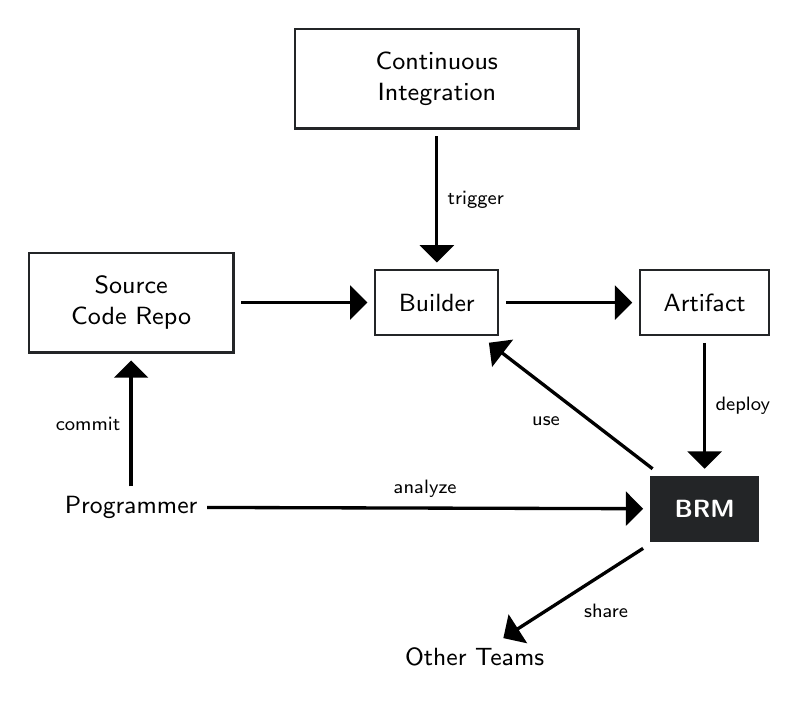
\begin{tikzpicture}
  \node[block, text width=2cm] (sources) {Source Code Repo};
  \node[block, right=of sources] (builder) {Builder};
  \node[block, above=of builder, text width=3cm] (ci) {Continuous Integration};
  \node[block, right=of builder] (artifact) {Artifact};
  \node[block, fill=myblack, text=white, below=of artifact] (brm) {\bfseries BRM};
  \node[below=of sources] (dev) {Programmer};
  \node[below left=of brm] (teams) {Other Teams};
  \path[ln]
    (sources) edge (builder)
    (ci) edge node {trigger} (builder)
    (builder) edge (artifact)
    (artifact) edge node {deploy} (brm)
    (brm) edge node {share} (teams)
    (dev) edge node {commit} (sources)
    (dev) edge node {analyze} (brm)
    (brm) edge node {use} (builder);
\end{tikzpicture}
\caption{The flow of data in an average software development team.}
\label{fig:map}
\end{figure}

The Section~\ref{sec:requirements} lists a few categories of existing
BRM solutions, analyses requirements their customers may have, and emphasize
the most important functional features and non-functional requirements.

\section{Requirements}
\label{sec:requirements}

All existing BRM solutions can be categorized as
public, commercial, hosted, open source, or surrogate.
Even though each of
them partially satisfy the needs of a professional software team, neither
one is perfect.

\begin{description}
  \item[Public]
  There are a few hosted BRMs for different programming languages, like
  \href{https://search.maven.org/}{Maven Central} for Java or
  \href{https://www.rubygems.org}{Rubygems} for Ruby, which are free to use,
  but do not allow private accounts. This means that all artifacts deployed
  by some user become available for all other users. This business model is
  acceptable for open source projects, but is not suitable for software teams
  that develop proprietary software products.

  \item[Commercial]
  There are a few BRMs, like
  \href{https://jfrog.com/artifactory/}{Artifactory}/\href{https://jfrog.com/bintray/}{Bintray}
  of \href{https://jfrog.com}{JFrog}
  and \href{https://www.sonatype.com/nexus-repository-oss}{Nexus}
  of \href{https://www.sonatype.com/}{Sonatype},
  which provide most of the features required by software teams, including
  fine-grained access control, versioning, seamless integration with build
  automation software, and many more. However, these tools are pretty expensive\footnote{%
    The annual cost of a license for a mid-size team of 50-100 developers is:
    \href{https://jfrog.com/pricing/}{around} \$30,000 for Artifactory
    and
    \href{https://www.sonatype.com/product-pricing}{around} \$50,000 for Nexus.
    There are less expensive products too:
    \href{https://inedo.com/proget/pricing}{ProGet} for \$10,000,
  }
  and require certain skills to install and manage them. Moreover, their
  authors (including JFrog and Sonatype) are US-based companies, who may be
  restricted to sell their products to software teams from certain ``sanctioned'' countries\footnote{%
    \href{https://techcrunch.com/2019/07/29/github-ban-sanctioned-countries/}{29th of July, 2019}:
    GitHub, the world's largest host of source code, is preventing users in Iran, Syria, Crimea.
    \href{https://techcrunch.com/2018/12/22/slack-says-it-will-comply-with-sanctions/}{22nd of December, 2018}:
    Slack confirms it will now block all activity in Iran and other sanctioned countries.
  }.

  \item[Hosted]
  There are a few BRMs, which maintain artifacts on their servers,
  like \href{https://www.cloudrepo.io/pricing.html}{CloudRepo} for Java
  or \href{https://pydist.com/}{PyDist} for Python.
  Some BRM creators, like JFrog, provide their products in hosted versions too.
  However, some software teams may not find this option accetable
  due to security reasons---eventually the data may be lost, if the company
  gets out of the market\footnote{%
    \href{https://www.theverge.com/2015/3/13/8206903/google-code-is-closing-down-github-bitbucket}{13th of March, 2015}:
    Google Code, one of the largest source code repository managers, closed its doors.
  }
  or due to sanctions.

  \item[Open source]
  There are also a few entirely free and open source products, like
  \href{https://archiva.apache.org/index.cgi}{Archiva}, which software
  teams must install, configure and use on their own risk. Even though
  this may sounds like a good solution for a small team, it may not be
  acceptable for a larger group of software developers, who expect their
  artifact repository to be reliable and available.

  \item[Surrogate]
  It is possible to organize a BRM without any software,
  \href{https://www.yegor256.com/2015/09/07/maven-repository-amazon-s3.html}{for example},
  on top of \href{https://aws.amazon.com/s3/}{Amazon S3}
  or a simple FTP server. With the right plugin
  Maven can deploy to Amazon S3 and then fetch artifacts from there
  via their built-in HTTP interface. However, such a solution gives
  very little or no control for a DevOps person and may only
  work for rather small software teams.
\end{description}

\subsection{Features}
\label{sec:features}

There are many important qualities and features software developers and DevOps
engineers expect a BRM to have, in order to be useful in a continuous
delivery pipeline. The most critical
\href{https://en.wikipedia.org/wiki/Non-functional_requirement}{non-functional requirements}
are:

\begin{description}
  \item[Integrability]
  There are plenty of build automation tools for each programming language,
  like \href{https://maven.apache.org/}{Maven} for Java,
  \href{https://www.npmjs.com/}{Npm} for JavaScript, or
  \href{https://github.com/ruby/rake}{Rake} for Ruby.
  There are also many continuous integration tools, like
  \href{https://jenkins.io/}{Jenkins} or \href{https://travis-ci.org/}{Travis}.
  Since automation is the most important aspect of DevOps, as noted by~\textcite{kerzazi2016},
  it is expected to have plugins for each or most of them, to enable seamless
  intregration with the BRM.

  \item[Availability]
  Artifacts are important components of a software development process
  and they must be available right when they are needed by a programmer
  or a build tool, without even small delays and delivered at the highest
  possible speed.

  \item[Scalability]
  Most build artifacts are large binary files. Some of them may even
  be larger than 1Gb, for example \href{https://www.docker.com/}{Docker}
  images or \dd{.war} production-ready Java archives.
  The BRM must be able to maintain large data sets, up to almost no limits.

  \item[Extensibility]
  It is highly desireable to have full access to the source code of the
  BRM and to have an ability to extend it with new plugins and modules. Moreover,
  vendor independence is important.

  \item[Reliability]
  An ability to corrupt the data due to software or harware failures must be
  eliminated, as much as it is possible.
\end{description}

\subsection{Non-functional Requirements}
\label{sec:nfr}

The most important \href{https://en.wikipedia.org/wiki/Functional_requirement}{functional requirements} are:

\begin{description}
  \item[Versions and Tags]
  New artifacts must not replace previously deployed ones.
  Instead, older versions must always be accessible. However,
  it is not expected that the BRM would assign version tags automatically,
  this is done at the pipeline's side.

  \item[Access Control]
  Larger teams may need to control who is allowed to use certain artifacts.
  Moreover, such teams may need to require the integration of authentication
  mechanisms of the BRM with the existing enterprise access-control system,
  via \href{https://en.wikipedia.org/wiki/Lightweight_Directory_Access_Protocol}{LDAP},
  for example. On top of regular access control, encryption mechanisms must
  be in place in order to prevent data leakage in case of software/hardware
  failures or human mistakes, as noted by~\textcite{paule2018}.

  \item[Analytics]
  Traceability between software artifacts is considered a very
  important factor in today development process, as noted by~\textcite{palihawadana2017}.
  BRM must make it possible to visualize dependencies between artifacts and
  operate on them.
\end{description}

There are many other essential features required, including
authentication and authorization, deployment, publishing,
download, removal, usage tracking, email notifications, mirroring,
and so on.

\subsection{Expected Metrics}
\label{ref:metrics}

In a large enterprise it is expected to have the following
numbers, in terms of load, size, and speed:

\begin{tabular}{ll}
Users, total & 80K \\
Artifacts hosted & 100M \\
New artifacts uploaded, daily & 10K \\
Data hosted & 100Tb \\
Data uploaded, daily & 10Gb \\
Concurrent connections, peek & 10 \\
Upload bandwidth, peek & 10M/s \\
Download bandwidth, peek & 100M/s \\
\end{tabular}

Smaller companies may have lower expectations.

\section{Architecture}



\section{Conclusion}
\label{sec:conclusion}

To be written...

\subsection{Acknowledgements}
\label{sec:ack}

The document was originally created by Yegor Bugayenko (y00538675).

\printbibliography%
\end{document}
